\documentclass[10pt, letterpaper, twocolumn]{article}

% =========================================================
% PAQUETES DE IDIOMA Y TIPOGRAFÍA
% =========================================================
\usepackage[utf8]{inputenc}
\usepackage[T1]{fontenc}
\usepackage{lmodern}
\usepackage[spanish, es-nodecimaldot]{babel}
\usepackage{microtype}

% =========================================================
% MÁRGENES Y FORMATO DE PÁGINA
% =========================================================
\usepackage[top=2cm, bottom=2cm, left=1.8cm, right=1.8cm, columnsep=0.65cm]{geometry}
\usepackage{setspace}
\spacing{1.05}

% =========================================================
% MATEMÁTICAS, TABLAS Y FIGURAS
% =========================================================
\usepackage{amsmath, amssymb, amsfonts}
\usepackage{graphicx}
\usepackage{booktabs}
\usepackage{caption}

% Enlaces hipertexto
\usepackage[colorlinks=true, allcolors=blue]{hyperref}

% =========================================================
% INICIO DEL DOCUMENTO
% =========================================================
\begin{document}

% ---------------------------------------------------------
% ENCABEZADO SUPERIOR A PÁGINA COMPLETA
% ---------------------------------------------------------
\twocolumn[{%
  % Fila superior: Escudos y Membrete Institucional
  \begin{minipage}{0.13\textwidth}
    \centering
    \IfFileExists{escudo_unam..png}{%
      
\includegraphics[width=\linewidth]{escudo_unam..png}%
    }{%
      \framebox[\linewidth]{\rule{0pt}{1.8cm}\footnotesize Escudo UNAM}%
    }
  \end{minipage}%
  \hfill
  \begin{minipage}{0.72\textwidth}
    \centering
    {\large\textbf{UNIVERSIDAD NACIONAL AUTÓNOMA DE MÉXICO}}\\[0.25em]
    {\small\textbf{FACULTAD DE CIENCIAS --- LICENCIATURA EN FÍSICA}}\\[0.25em]
    {\footnotesize\textbf{Laboratorio de Fenómenos Colectivos} \quad|\quad Semestre 2027-1}
  \end{minipage}%
  \hfill
  \begin{minipage}{0.13\textwidth}
    \centering
    \IfFileExists{escudo_ciencias.png}{%
      
\includegraphics[width=\linewidth]{escudo_ciencias.png}%
    }{%
      \framebox[\linewidth]{\rule{0pt}{1.8cm}\footnotesize Escudo FC}%
    }
  \end{minipage}

  \vspace{0.35cm}
  \hrule height 0.8pt
  \vspace{0.45cm}

  % Título, autor y datos del curso
  \begin{center}
    {\Large\bfseries Práctica 1: Determinación de la densidad.}\\[0.6em]
    
    {\normalsize \textbf{Barrientos Clemente Juan Alfredo}}\\[0.2em]
    {\footnotesize \textit{Facultad de Ciencias, Universidad Nacional Autónoma de México}}\\[0.2em]
    
    {\footnotesize \textbf{Profesoras:} Dra. Reyna Guadalupe Ramírez De la Torre, Fís. Ximena Fernández de Córdoba Montenegro \quad $\cdot$ \quad \textbf{Grupo:} 8161}\\[0.2em]
    {\footnotesize  \quad \textit{Fecha de entrega:} 09/09/2026}
  \end{center}

  \vspace{0.25cm}

  % Resumen estructurado según la guía (5-10 líneas)
  \begin{quotation}
    \small
    \noindent\textbf{Resumen}--- En esta practica se determinó experimentalmente la densidad de diversos materiales mediante tres métodos: la medición geométrica directa con análisis de sensibilidad instrumental en un alambre continuo, la caracterización colectiva mediante ajuste por mínimos cuadrados en conjuntos de cilindros y la estimación poblacional por muestreo. Se obtuvo una densidad experimental de $\bar{\rho} = 8.60 \pm 0.131\ \mathrm{g/cm^3}$ para el alambre de cobre. A través del análisis gráfico y el estudio de cilindros individuales se identificaron con éxito especímenes de latón, aluminio y cobre, contrastando las desviaciones frente a los valores teóricos a excepcion del policatbonoto, que tal vez aea otro material. Finalmente, mediante el muestreo estadístico de cacahuates, se estimó una población de $N = 736 \pm 52$ piezas en una bolsa de $850\ \mathrm{g}$. 
    \vspace{0.35em}

  \end{quotation}

  \vspace{0.35cm}
  \hrule height 0.4pt
  \vspace{0.55cm}
}]

% ---------------------------------------------------------
% CUERPO DEL ARTÍCULO (A DOS COLUMNAS)
% ---------------------------------------------------------

\section{Introducción}
La densidad ($\rho$) es una propiedad esencial para la caracterización mecánica y termodinámica de materiales. En este trabajo se abordan tres metodos complementarios de estimación física:
\begin{enumerate}
    \item Determinación geométrica directa y análisis de sensibilidad instrumental en un alambre continuo.
    \item Determinación colectiva mediante ajuste por mínimos cuadrados en conjuntos de cilindros metálicos homogéneos y heterogéneos.
    \item Estimación poblacional de sistemas de particulados discretos.
\end{enumerate}

\subsection{Hipótesis de los modelos}
Asumimos que los cuerpos sólidos presentan una geometría cilíndrica ideal, libre de deformaciones macroscópicas, y una distribución homogénea de la masa. Como hipótesis postulamos que tanto el alambre como el conjunto de once cilindros están constituidos de cobre, mientras que el grupo de cuatro cilindros diversos comprende piezas de latón, aluminio, cobre y policarbonato. Tambien, para el muestreo discreto, se asume que la muestra de diez cacahuates es estadísticamente representativa de la distribución poblacional total de la bolsa, asi que en promedio puede haber 850 cacahuates en la bolsa, asumiedo que cada uno pese $1g$

\section{Marco Teórico}
\subsection{Densidad individual y propagación}
Para un alambre de longitud $L$, masa $m$ y diámetro $d$:
\begin{equation}
    \rho = \frac{m}{\left(\frac{d}{2}\right)^2\pi L}.
    \label{eq:densidad_alambre}
\end{equation}
La propagación de incertidumbres independientes lleva a:
\begin{equation}
    \frac{\delta \rho}{\rho} = \sqrt{\left(\frac{\delta m}{m}\right)^2 + \left(\frac{\delta L}{L}\right)^2 + \left(2\,\frac{\delta d}{d}\right)^2}.
    \label{eq:error_relativo}
\end{equation}

\subsection{Ajuste lineal para conjuntos de sólidos}
La relación funcional $m(V) = \rho V$ que permite plantear el modelo de regresión:
\begin{equation}
    m_i = \rho_{\mathrm{ajuste}} V_i + b,
    \label{eq:lineal}
\end{equation}
donde la pendiente minimiza las discrepancias aleatorias de las mediciones geométricas individuales y $b \approx 0$ nos valida que no haya errores sistemáticos de masa.

\subsection{Densidad de cilindros diversos y discriminación de materiales}
Se seleccionaron cuatro muestras representativas para determinar su densidad experimental y contrastarla con los valores teóricos de referencia planteados en la hipótesis inicial: latón, aluminio, cobre y plástico

\subsection{Muestreo discreto}
Para una masa neta $M_{\mathrm{total}}$ y una muestra de $n$ unidades con masa promedio $\bar{m}_c=850g$:
\begin{equation}
    N = \frac{M_{\mathrm{total}}}{\bar{m}_c}, \quad \delta N = N \sqrt{\left(\frac{\delta M_{\mathrm{total}}}{M_{\mathrm{total}}}\right)^2 + \left(\frac{\delta \bar{m}_c}{\bar{m}_c}\right)^2}.
    \label{eq:cacahuates}
\end{equation}

\section{Desarrollo Experimental}
Se empleó una balanza electrónica ($\pm 0.0001\,\mathrm{g}$), balanza digital($\pm 0.05\,\mathrm{g}$), regla ($\pm 0.5\,\mathrm{cm}$), vernier digital ($\pm 0.001\,\mathrm{mm}$) y micrómetro digital  ($\pm 0.001\,\mathrm{mm}$).

\subsection{Alambre metálico}
La masa y la longitud del alambre se determinaron mediante una balanza y una regla, respectivamente. Para evaluar el impacto de la resolución en la incertidumbre propagada, se efectuaron $N=12$ mediciones del diámetro empleando un vernier y un micrómetro.

\subsection{Cilindros}
Se determinaron experimentalmente la masa y las dimensiones geométricas (altura y diámetro, medidas mediante un vernier) de 11 cilindros iniciales. Posteriormente, se realizaron las mismas mediciones en cuatro cilindros, clasificados según el material aparente de cada muestra.

\subsection{Muestra discreta}
Se nos dieron aleatoriamente 10 cacahuates japonés, registrando sus masas y diametros individuales en la balanza y vernier.

\section{Resultados y Análisis}

\subsection{Densidad del alambre y selección de instrumental}
Para reducir el impacto de las fluctuaciones aleatorias, se hicieron $N=12$ mediciones independientes tanto de la masa como del diámetro a lo largo del alambre. Tras procesar estadísticamente este conjunto de datos y propagar las incertidumbres correspondientes a los instrumentos utilizados, se determinaron los valores promedio del volumen y la densidad, cuyos resultados consolidados se presentan en la Tabla~\ref{tab:densidad_alambre}.\\
En la Gráfica~\ref{fig:comparacion_densidad} vamos a notar que nos aproximamos mucho al valor real del cobre, tal vez no estamos dentro de la linea roja poque tal vez nuestro alambre este recubierto por un esmalte aislante o sea alguna aleacion de cobre con algún otro metal que mejore sus propiedades
\begin{table}[htbp]
    \centering
    \resizebox{\columnwidth}{!}{%
    \begin{tabular}{cccc}
        \toprule
        \textbf{$\bar{d}$ [$\mathrm{mm}$]} & \textbf{$\bar{m}$ [$\mathrm{g}$]} & \textbf{$\bar{V}$ [$\mathrm{cm^3}$]} & \textbf{$\bar{\rho}$ [$\mathrm{g/cm^3}$]} \\
        \midrule
        $0.649 \pm 2.89 \times 10^{-4}$ & $0.9380 \pm 6.4 \times 10^{-5}$ & $0.1092 \pm 0.0017$ & $8.60 \pm 0.131$ \\
        \bottomrule
    \end{tabular}%
    }
    \centering
    \caption{Promedios geométricos, masa y densidad final del alambre.}
    \label{tab:densidad_alambre}
\end{table}
\begin{figure}[htbp]
    \centering
    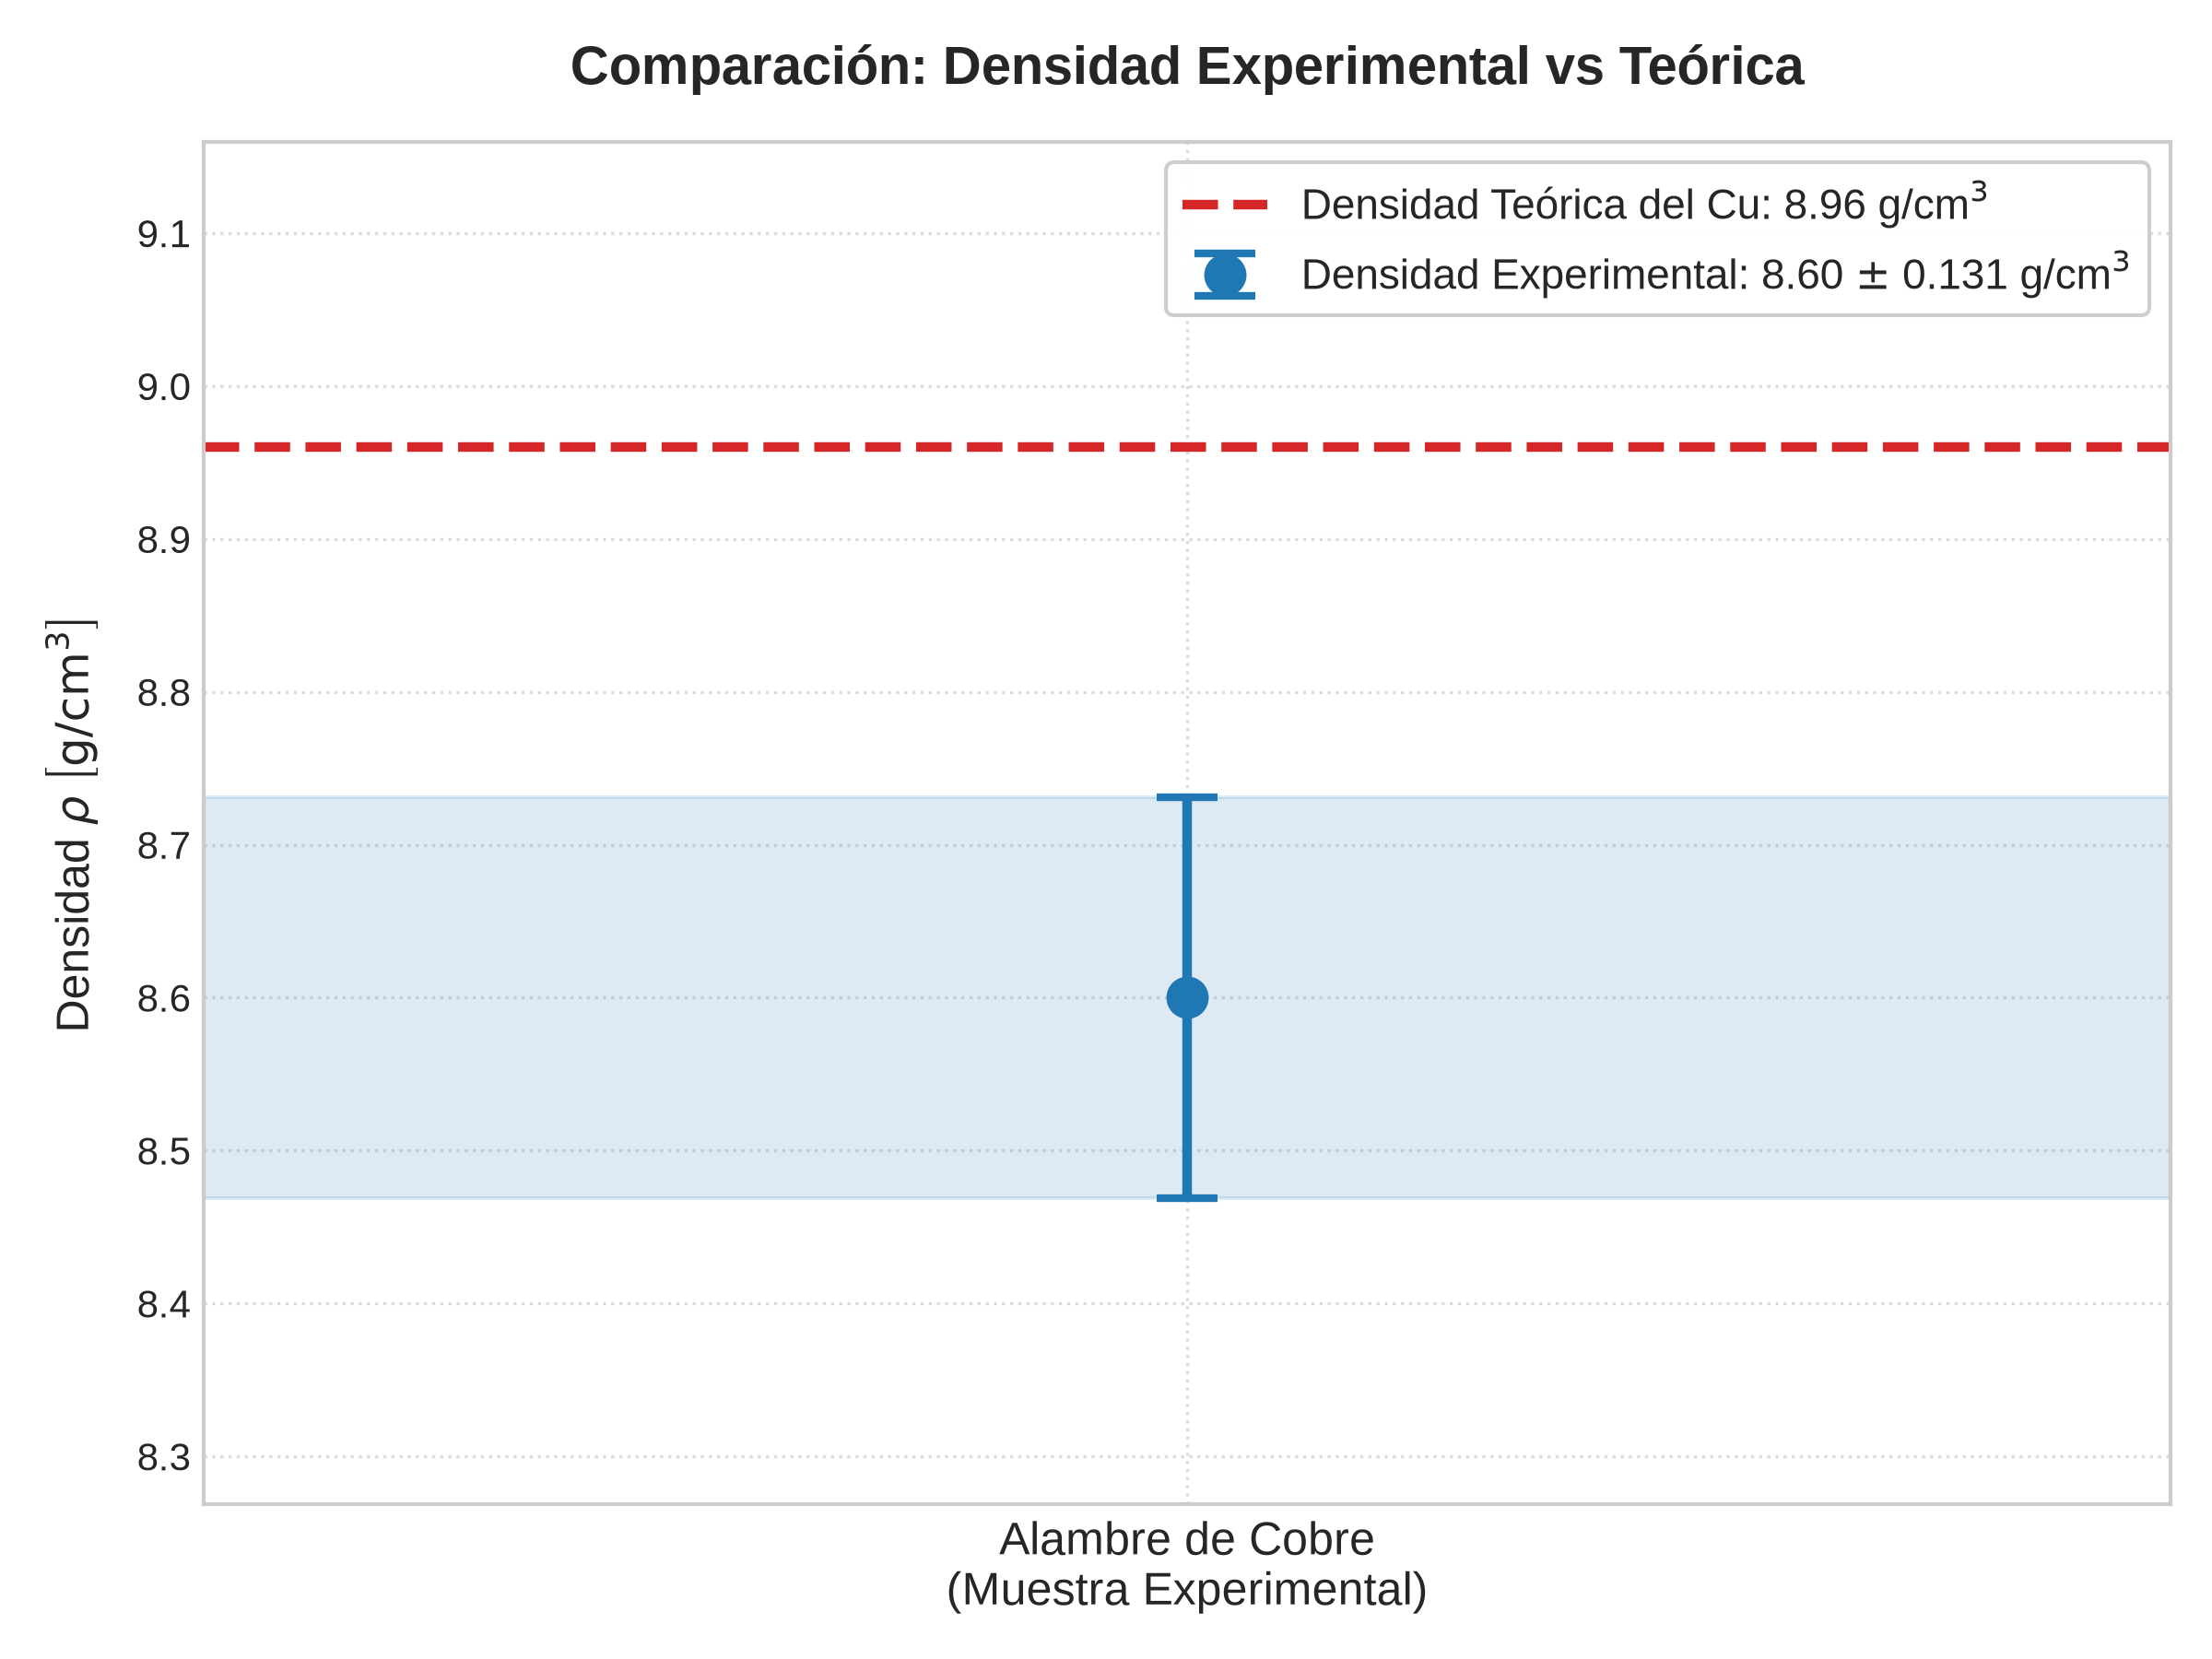
\includegraphics[width=\linewidth]{comparacion_densidad.png}
    \caption{Comparación entre la densidad experimental obtenida para el alambre y el valor teórico de referencia para el cobre. Lo sombreado representa la incertidumbre experimental propagada.}
    \label{fig:comparacion_densidad}
\end{figure}

\subsection{Regresión lineal y clasificación de cilindros}
Para caracterizar la densidad a nivel colectivo y minimizar los errores aleatorios de mediciones aisladas, se determinaron la masa y el volumen de 11 cilindros metálicos. Inicialmente, se aplicó un modelo de regresión lineal global bajo la hipótesis de que todas las piezas compartían la misma composición; no obstante, la alta dispersión de los residuales en el plano masa-volumen evidenció la heterogeneidad de la muestra. En consecuencia, los especímenes se estratificaron empíricamente en cuatro grupos físicamente homogéneos. En la Figura~\ref{fig:11cilindros} se ilustra el comportamiento gráfico de esta segmentación. Asimismo, la Tabla~\ref{tab:densidades_individuales} adjunta resume las incertidumbres y los parámetros del ajuste lineal por mínimos cuadrados, cuya pendiente ($\rho_{\mathrm{ajuste}}$) fungió como el valor decisivo para identificar el material de manera concluyente.

\begin{figure}[htbp]
    \centering
    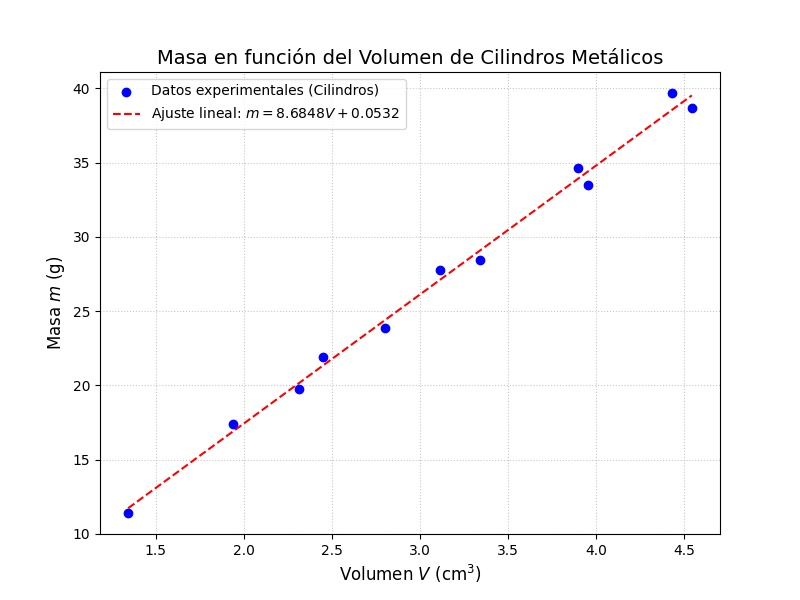
\includegraphics[width=\linewidth]{masa-volumen.png}
    \caption{Regresión lineal global de masa en función del volumen para el conjunto inicial de 11 cilindros metálicos.}
    \label{fig:11cilindros}
\end{figure}

\begin{table}[htbp]
    \centering
    \caption{Densidades calculadas individualmente para el conjunto de 11 cilindros metálicos.}
    \label{tab:densidades_individuales}
    \begin{tabular}{cc}
        \toprule
        \textbf{Cilindro} & \textbf{Densidad $\rho$ [$\mathrm{g/cm^3}$]} \\
        \midrule
        cil\_1  & $8.4845 \pm 0.0373$ \\
        cil\_2  & $8.9750 \pm 0.0259$ \\
        cil\_3  & $8.5367 \pm 0.0218$ \\
        cil\_4  & $8.9400 \pm 0.0206$ \\
        cil\_5  & $8.5173 \pm 0.0181$ \\
        cil\_6  & $8.9133 \pm 0.0164$ \\
        cil\_7  & $8.5204 \pm 0.0154$ \\
        cil\_8  & $8.8930 \pm 0.0135$ \\
        cil\_9  & $8.4716 \pm 0.0133$ \\
        cil\_10 & $8.9400 \pm 0.0123$ \\
        cil\_11 & $8.5035 \pm 0.0111$ \\
        \bottomrule
    \end{tabular}
    

\end{table}

Como se observa en la Figura~\ref{fig:11cilindros}, la recta de ajuste general no representa de manera adecuada al conjunto de datos. La notable dispersión de los puntos experimentales (algunos sistemáticamente por encima o por debajo de la tendencia lineal) invalida la hipótesis inicial de que todos los cilindros están fabricados con el mismo material (cobre puro).\\
Para complementar el análisis colectivo y corroborar la composición específica de los materiales, se tomaron cuatro cilindros representativos correspondientes a distintos materiales (latón, Tabla~\ref{tab:cil_laton}; aluminio, Tabla~\ref{tab:cil_aluminio}; cobre, Tabla~\ref{tab:cil_cobre} y plástico, Tabla~\ref{tab:cil_plastico}). Con el fin de minimizar fluctuaciones aleatorias, a cada cilindro se le aplicó un muestreo repetido de sus dimensiones geométricas empleando el vernier y balanza digital. A partir del tratamiento estadístico de estas mediciones empíricas y la propagación analítica de las incertidumbres instrumentales, se determinó el volumen y la densidad volumétrica individual de cada pieza. Los parámetros consolidados resultantes de este proceso se exponen a continuación.

\begin{table}[htbp]
    \centering
    \caption{Parámetros geométricos, masa y densidad empírica para el cilindro de Latón.}
    \label{tab:cil_laton}
    \begin{tabular}{lc}
        \toprule
        \textbf{Magnitud} & \textbf{Valor e Incertidumbre} \\
        \midrule
        Diámetro $d$ & $1.0037 \pm 0.0003\,\mathrm{cm}$ \\
        Altura $h$ & $1.2080 \pm 0.0031\,\mathrm{cm}$ \\
        Masa $m$ & $8.0600 \pm 0.0500\,\mathrm{g}$ \\
        Volumen $V$ & $0.9557\,\mathrm{cm^3}$ \\
        Densidad $\rho$ & $8.433 \pm 0.057\,\mathrm{g/cm^3}$ \\
        \bottomrule
    \end{tabular}
\end{table}

\begin{table}[htbp]
    \centering
    \caption{Parámetros geométricos, masa y densidad empírica para el cilindro de Aluminio.}
    \label{tab:cil_aluminio}
    \begin{tabular}{lc}
        \toprule
        \textbf{Magnitud} & \textbf{Valor e Incertidumbre} \\
        \midrule
        Diámetro $d$ & $1.0027 \pm 0.0003\,\mathrm{cm}$ \\
        Altura $h$ & $1.2000 \pm 0.0001\,\mathrm{cm}$ \\
        Masa $m$ & $2.5467 \pm 0.0501\,\mathrm{g}$ \\
        Volumen $V$ & $0.9475\,\mathrm{cm^3}$ \\
        Densidad $\rho$ & $2.688 \pm 0.053\,\mathrm{g/cm^3}$ \\
        \bottomrule
    \end{tabular}
\end{table}

\begin{table}[htbp]
    \centering
    \caption{Parámetros geométricos, masa y densidad empírica para el cilindro de Cobre.}
    \label{tab:cil_cobre}
    \begin{tabular}{lc}
        \toprule
        \textbf{Magnitud} & \textbf{Valor e Incertidumbre} \\
        \midrule
        Diámetro $d$ & $0.9953 \pm 0.0003\,\mathrm{cm}$ \\
        Altura $h$ & $1.2010 \pm 0.0006\,\mathrm{cm}$ \\
        Masa $m$ & $8.3267 \pm 0.0501\,\mathrm{g}$ \\
        Volumen $V$ & $0.9345\,\mathrm{cm^3}$ \\
        Densidad $\rho$ & $8.910 \pm 0.054\,\mathrm{g/cm^3}$ \\
        \bottomrule
    \end{tabular}
\end{table}

\begin{table}[htbp]
    \centering
    \caption{Parámetros geométricos, masa y densidad empírica para el cilindro de Plástico.}
    \label{tab:cil_plastico}
    \begin{tabular}{lc}
        \toprule
        \textbf{Magnitud} & \textbf{Valor e Incertidumbre} \\
        \midrule
        Diámetro $d$ & $0.9927 \pm 0.0003\,\mathrm{cm}$ \\
        Altura $h$ & $1.2017 \pm 0.0003\,\mathrm{cm}$ \\
        Masa $m$ & $1.0700 \pm 0.0500\,\mathrm{g}$ \\
        Volumen $V$ & $0.9300\,\mathrm{cm^3}$ \\
        Densidad $\rho$ & $1.151 \pm 0.054\,\mathrm{g/cm^3}$ \\
        \bottomrule
    \end{tabular}
\end{table}
La comparación de las densidades experimentales con los valores teóricos de referencia se resume en la Tabla~\ref{tab:comparacion_individual}. Los metales muestran una excelente concordancia con la teoría, mientras que el plástico presenta una gran discrepancia, lo que nos podria sugerir una composición distinta a la esperada o que sea otro material.


Para evaluar la exactitud de las determinaciones geométricas individuales, las densidades empíricas se contrastaron con los valores teóricos de referencia esperados. El análisis de discrepancia se resume en la Tabla~\ref{tab:comparacion_individual}.
\begin{table}[htbp]
    \centering
    \caption{Comparación analítica entre las densidades experimentales y los valores teóricos de referencia.}
    \label{tab:comparacion_individual}
    \resizebox{\columnwidth}{!}{%
    \begin{tabular}{lcccc}
        \toprule
        \textbf{Material} & \textbf{$\rho_{\mathrm{exp}}$ [$\mathrm{g/cm^3}$]} & \textbf{$\rho_{\mathrm{teo}}$ [$\mathrm{g/cm^3}$]} \\
        \midrule
        Latón    & $8.433 \pm 0.057$ & $8.40$ -- $8.70$  \\
        Aluminio & $2.688 \pm 0.053$ & $2.70$           \\
        Cobre    & $8.910 \pm 0.054$ & $8.96$           \\
        Plástico (Policarb.) & $1.151 \pm 0.054$ & $1.30$ \\
        \bottomrule
    \end{tabular}%
    }
    
\end{table}




\subsection{Estimación poblacional de cacahuates}
Con el propósito de extrapolar propiedades macroscópicas a partir de sistemas discretos heterogéneos, se analizó una muestra representativa de 10 cacahuates. Mediante mediciones individuales (masa), se evaluó la variabilidad en masa y dimensiones para estimar el número total de piezas en una bolsa de $850\,\mathrm{g}$. Los registros experimentales de la muestra se detallan en la Tabla~\ref{tab:cacahuates}.

\begin{table}[htbp]
    \centering
    \caption{Mediciones individuales de masa y diámetro para la muestra de 10 cacahuates japoneses.}
    \label{tab:cacahuates}
    \begin{tabular}{ccc}
        \toprule
        \textbf{Muestra ($n$)} & \textbf{Masa $m$ [$\mathrm{g}$]} & \textbf{Diámetro $d$ [$\mathrm{mm}$]} \\
        \midrule
        1  & $1.20$ & $1.72$ \\
        2  & $1.15$ & $3.12$ \\
        3  & $1.39$ & $1.75$ \\
        4  & $0.86$ & $0.64$ \\
        5  & $0.96$ & $1.05$ \\
        6  & $1.16$ & $1.88$ \\
        7  & $1.40$ & $1.79$ \\
        8  & $1.44$ & $1.12$ \\
        9  & $0.91$ & $0.70$ \\
        10 & $1.08$ & $2.98$ \\
        \bottomrule
    \end{tabular}
\end{table}
utilizando la ecuacion~\ref{eq:cacahuates} obtuvimos que habian, aproximadamente, $N=736 \pm 52$ cacahuates de 767
\section{Conclusiones}
Se cumplieron satisfactoriamente los objetivos planteados, ya que las muestras analizadas resultaron ser cobre, aluminio y latón, con excepción del plástico, que parece corresponder a un tipo más específico de este material.

A partir de las mediciones y del análisis de los datos, pudimos comprobar la importancia de utilizar instrumentos con muy alta resolución, como el micrómetro y el vernier, porque permiten reducir la incertidumbre en las mediciones. Esto fue muy útil para comprobar que la densidad obtenida para el alambre se encuentra cercana al valor teórico del cobre.

También notamos que el uso de una regresión lineal permite obtener resultados más confiables que simplemente calcular un promedio, especialmente cuando se trabaja con sólidos y existen variaciones en las mediciones. Esto facilitó la identificación de los diferentes materiales.

Finalmente, el método utilizado para contar la muestra de los diez cacahuates permitió estimar de manera aproximada la cantidad total contenida en la bolsa, obteniendo un resultado de $N = 736 \pm 52$ cacahuates para una bolsa de $850\ \mathrm{g}$.

\section{Bibliografia}
@misc{colaboradores-de-wikipedia-2026,
	author = {colaboradores de Wikipedia},
	month = {2},
	title = {{Latón}},
	year = {2026},
	url = {https://es.wikipedia.org/wiki/Lat%C3%B3n},
}
@misc{unknown-author-no-date,
	title = {{Aluminio (Al) Propiedades químicas y efectos sobre la salud y el medio ambiente}},
	url = {https://www.lenntech.es/periodica/elementos/al.htm},
}
@misc{colaboradores-de-wikipedia-2025,
	author = {colaboradores de Wikipedia},
	month = {4},
	title = {{Policarbonato}},
	year = {2025},
	url = {https://es.wikipedia.org/wiki/Policarbonato},
}
\end{document}